\chapter{\textbf{Phân quyền và kiểm soát truy cập}}
\section{Phân quyền cho máy in bằng ICACLS}
\begin{lstlisting}[style=powershell]
$Domain = "ABC"
 
# Configure printer permissions
$PermissionConfig = @(
    @{Name="PRN_Design_01"; Group="GRP_Design"},
    @{Name="PRN_Design_02"; Group="GRP_Design"},
    @{Name="PRN_Office_01"; Group="GRP_Office"},
    @{Name="PRN_Office_02"; Group="GRP_Office"},
    @{Name="PRN_Office_03"; Group="GRP_Office"},
    @{Name="PRN_Accounting_01"; Group="GRP_Accounting"},
    @{Name="PRN_Accounting_02"; Group="GRP_Accounting"}
)
 
foreach ($printer in $PermissionConfig) {
    Write-Host "Configuring: $($printer.Name)" -ForegroundColor Cyan
    
    # Grant permissions using icacls
    & icacls "\\.\pipe\$($printer.Name)" /inheritance:r `
        /grant:f "${Domain}\$($printer.Group):(OI)(CI)(F)" `
        /grant:f "SYSTEM:(OI)(CI)(F)" `
        /grant:f "Administrators:(OI)(CI)(F)" 2>$null
        
    Write-Host "  [OK] Done" -ForegroundColor Green
}
 
# Configure Pool permissions
Write-Host "Configuring: PRN_Pool_Office" -ForegroundColor Cyan
 
& icacls "\\.\pipe\PRN_Pool_Office" /inheritance:r `
    /grant:f "${Domain}\GRP_Design:(OI)(CI)(F)" `
    /grant:f "${Domain}\GRP_Office:(OI)(CI)(F)" `
    /grant:f "${Domain}\GRP_Accounting:(OI)(CI)(F)" `
    /grant:f "SYSTEM:(OI)(CI)(F)" `
    /grant:f "Administrators:(OI)(CI)(F)" 2>$null
    
Write-Host "  [OK] Done" -ForegroundColor Green
\end{lstlisting}

\begin{figure}[htbp]
    \centering
    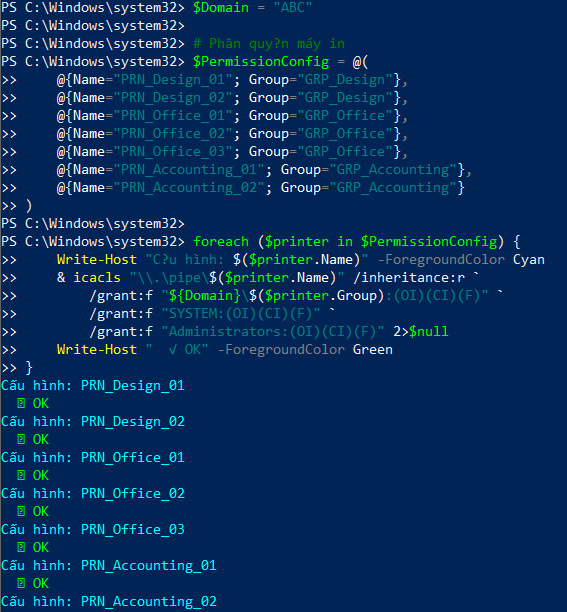
\includegraphics[width=0.75\textwidth]{./media/PHÂN QUYỀN CHO MÁY IN.png}
    \vspace{-0.3cm}
    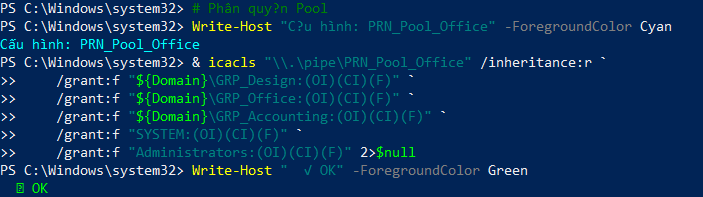
\includegraphics[width=0.75\textwidth]{./media/PHÂN QUYỀN CHO MÁY IN(1).png}
    \caption{Phân quyền cho máy in}
    \label{fig:mirrored_vd_19}
\end{figure}

\noindent\textbf{Giải thích tham số:}
\begin{itemize}[topsep=2pt,itemsep=1pt,parsep=0pt]
    \item (OI): Object Inherit – quyền áp dụng cho đối tượng con khi có.
    \item (CI): Container Inherit – quyền áp dụng cho container con.
    \item (F): Full control – toàn quyền sử dụng.
\end{itemize}

\noindent\textit{Các nhóm user AD (Active Directory):}
\begin{itemize}[topsep=2pt,itemsep=1pt,parsep=0pt]
    \item \textit{GRP\_Design\_Users: Chỉ được dùng máy in của phòng thiết kế và máy in pool.}
    \item \textit{GRP\_Office\_Users: Chỉ được dùng máy in của phòng văn phòng và máy in pool.}
    \item \textit{GRP\_Accounting\_Users: Chỉ được dùng máy in của phòng kế toán và máy in pool.}
\end{itemize}

\begin{table}[htbp]
    \centering
    \caption{Phân quyền máy in theo nhóm}
    \label{tab:printer_permissions}
    \begin{tabular}{|l|l|p{4.5cm}|}
        \hline
        \textbf{Tên máy in} & \textbf{Nhóm được cấp quyền} & \textbf{Mô tả quyền} \\ \hline
        PRN\_Design\_Color\_01 & GRP\_Design\_Users & Toàn quyền phòng thiết kế \\ \hline
        PRN\_Office\_BW\_01 & GRP\_Office\_Users & Toàn quyền phòng văn phòng \\ \hline
        PRN\_Accounting\_BW\_01 & GRP\_Accounting\_Users & Toàn quyền phòng kế toán \\ \hline
        PRN\_Pool\_General & Cả 3 nhóm phòng ban & Dùng chung, chia tải \\ \hline
    \end{tabular}
\end{table}

\section{Thiết lập độ ưu tiên cho các máy in (Priority)}
\begin{lstlisting}[style=powershell]
$PriorityConfig = @(
    @{Printer="PRN_Design_01"; Priority=50},
    @{Printer="PRN_Design_02"; Priority=50},
    @{Printer="PRN_Office_01"; Priority=25},
    @{Printer="PRN_Office_02"; Priority=25},
    @{Printer="PRN_Office_03"; Priority=25},
    @{Printer="PRN_Pool_Office"; Priority=30},
    @{Printer="PRN_Accounting_01"; Priority=75},
    @{Printer="PRN_Accounting_02"; Priority=75}
)

foreach ($config in $PriorityConfig) {
    try {
        Set-Printer -Name $config.Printer -Priority $config.Priority -ErrorAction Stop
        Write-Host "[OK] $($config.Printer) - Priority: $($config.Priority)" -ForegroundColor Green
    } catch {
        Write-Host "[!] Error setting priority $($config.Printer): $_" -ForegroundColor Yellow
    }
}

# Check priority
Write-Host "`n--- Priority List ---" -ForegroundColor Cyan
Get-Printer | Where-Object {$_.Name -like "PRN_*"} | Select-Object Name, Priority | Format-Table
\end{lstlisting}

\begin{figure}[htbp]
    \centering
    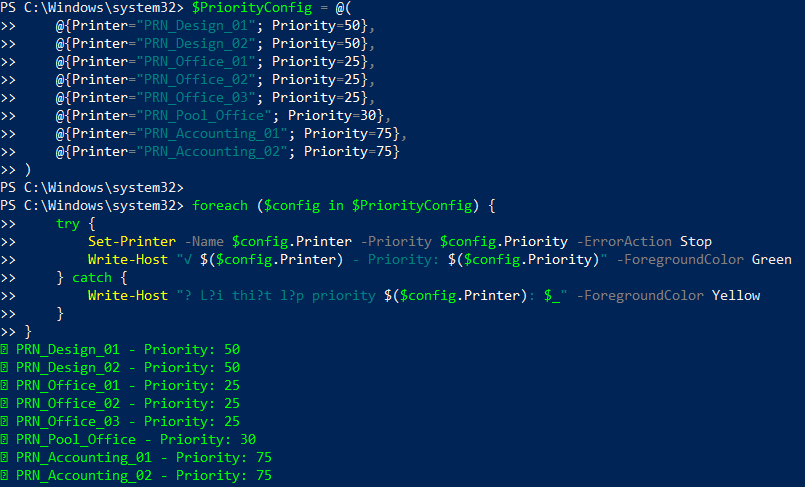
\includegraphics[width=0.7\textwidth]{./media/THIẾT LẬP ĐỘ ƯU TIÊN CHO MÁY IN.png}
    \vspace{-0.3cm}
    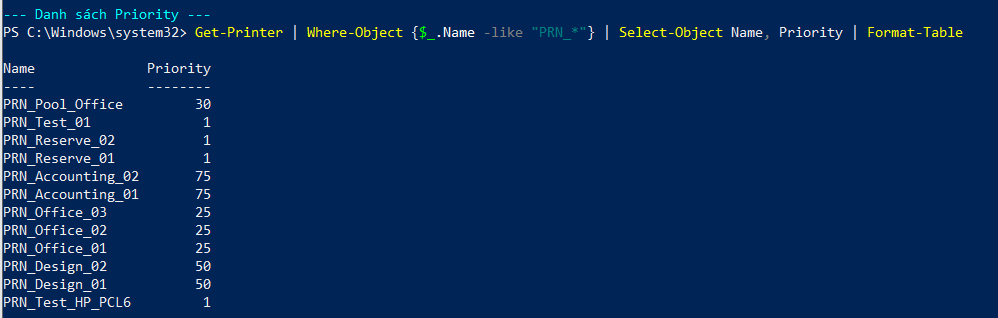
\includegraphics[width=0.7\textwidth]{./media/THIẾT LẬP ĐỘ ƯU TIÊN CHO MÁY IN(1).png}
    \caption{Thiết lập độ ưu tiên cho các máy in}

    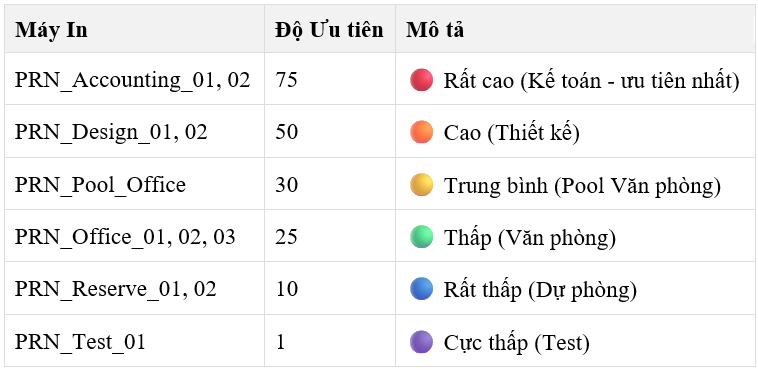
\includegraphics[width=0.85\textwidth]{./media/DUT.png}
    \caption{Độ ưu tiên của các máy in}
    \label{fig:mirrored_vd_16}
\end{figure}
\vspace{\baselineskip}


\chapter{\textbf{Phân phối máy in qua Group Policy}}
\section{Tạo Logon Script}
\begin{lstlisting}[style=powershell]
# Client Printer Deployment Script
$ClientDeployScript = @'
# Script runs on Client Windows 8.1 (Logon Script)
# Purpose: Automatically connect printers based on user AD group
 
Write-Host "=== Deploying Printers for User ===" -ForegroundColor Cyan
 
# Get current user information
$CurrentUser = [System.Security.Principal.WindowsIdentity]::GetCurrent().Name
Write-Host "Current User: $CurrentUser" -ForegroundColor Green
 
# Get user AD groups
$UserGroups = @()
try {
    $SamAccount = $CurrentUser.Split("\")[-1]
    $ADUser = Get-ADUser -Identity $SamAccount -Properties MemberOf -ErrorAction Stop
    $UserGroups = $ADUser.MemberOf | ForEach-Object {
        (Get-ADGroup -Identity $_ -ErrorAction SilentlyContinue).Name
    }
    Write-Host "User Groups: $($UserGroups -join ', ')" -ForegroundColor Green
} catch {
    Write-Host "Warning: Could not retrieve AD groups: $_" -ForegroundColor Yellow
}
 
# Define printers by group
$PrinterMapping = @{
    "GRP_Design" = @("\\SRV-PRINT\PRN_Design_01", "\\SRV-PRINT\PRN_Design_02");
    "GRP_Office" = @("\\SRV-PRINT\PRN_Office_01", "\\SRV-PRINT\PRN_Office_02", "\\SRV-PRINT\PRN_Office_03", "\\SRV-PRINT\PRN_Pool_Office");
    "GRP_Accounting" = @("\\SRV-PRINT\PRN_Accounting_01", "\\SRV-PRINT\PRN_Accounting_02")
}
 
# Connect printers matching user group
$ConnectedPrinters = @()
foreach ($group in $UserGroups) {
    if ($PrinterMapping.ContainsKey($group)) {
        Write-Host "Processing group: $group" -ForegroundColor Cyan
        foreach ($printer in $PrinterMapping[$group]) {
            try {
                Add-Printer -ConnectionName $printer -ErrorAction Stop
                $ConnectedPrinters += $printer
                Write-Host "[OK] Connected printer: $printer" -ForegroundColor Green
            } catch {
                Write-Host "[!] Failed to connect $printer : $_" -ForegroundColor Yellow
            }
        }
    }
}
 
# Display list of connected printers
Write-Host "`n=== Available Printers ===" -ForegroundColor Cyan
Get-Printer | Where-Object {$_.Type -eq "Connection"} | Select-Object Name, ComputerName | Format-Table -AutoSize
 
Write-Host "[OK] Printer deployment completed for $CurrentUser" -ForegroundColor Green
'@
 
# Save client script
$ScriptPath = "C:\PrinterScripts"
if (-not (Test-Path $ScriptPath)) {
    New-Item -ItemType Directory -Path $ScriptPath -Force | Out-Null
    Write-Host "[OK] Created folder $ScriptPath" -ForegroundColor Green
}
 
$ClientScriptFile = "$ScriptPath\Deploy-Printers-Client.ps1"
$ClientDeployScript | Out-File -FilePath $ClientScriptFile -Encoding UTF8 -Force
Write-Host "[OK] Client script saved at: $ClientScriptFile" -ForegroundColor Green
 
# Share script folder for client download
Write-Host "`n--- Share Script Folder ---" -ForegroundColor Cyan
 
$ShareName = "PrinterScripts"
try {
    New-SmbShare -Name $ShareName -Path $ScriptPath -FullAccess "Authenticated Users" -ErrorAction Stop
    Write-Host "[OK] Folder $ShareName shared successfully" -ForegroundColor Green
} catch {
    Write-Host "[!] Folder $ShareName already shared or error: $_" -ForegroundColor Yellow
}
\end{lstlisting}

\begin{figure}[htbp]
    \centering
    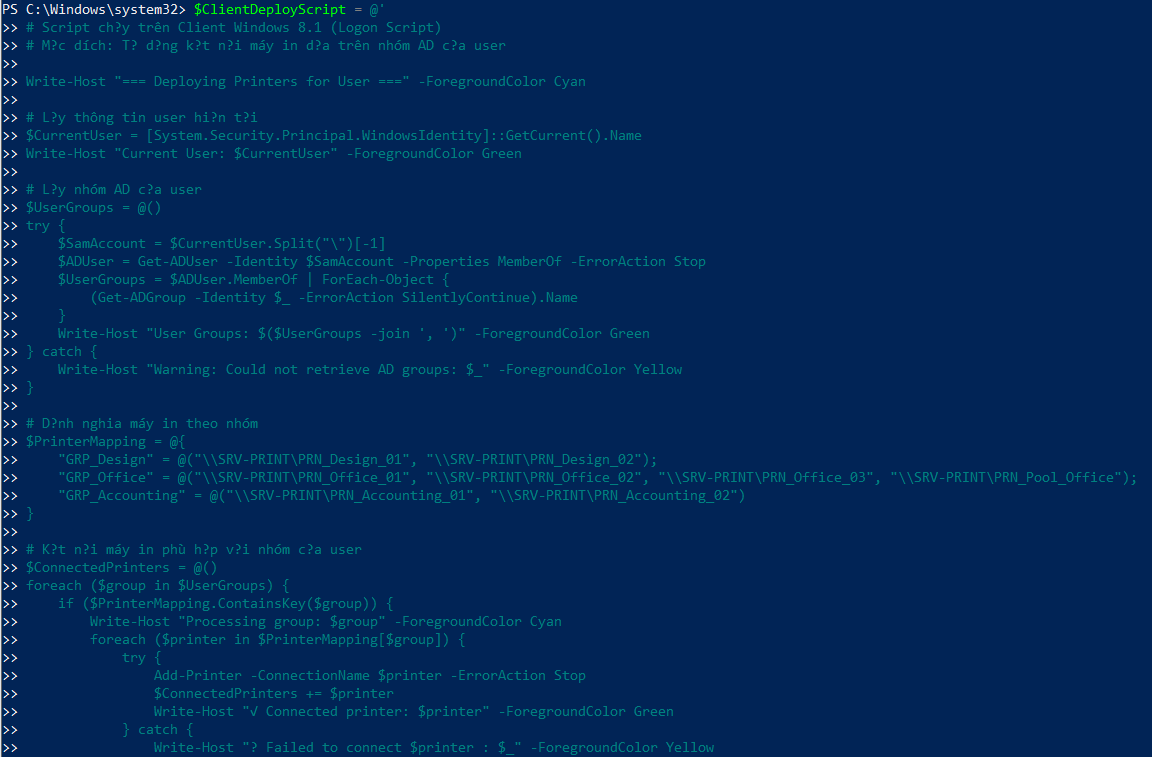
\includegraphics[width=0.7\textwidth]{./media/TẠO SCRIPT PHÂN PHỐI MÁY IN ĐẾN CLIENT.png}
    \vspace{-0.25cm}
    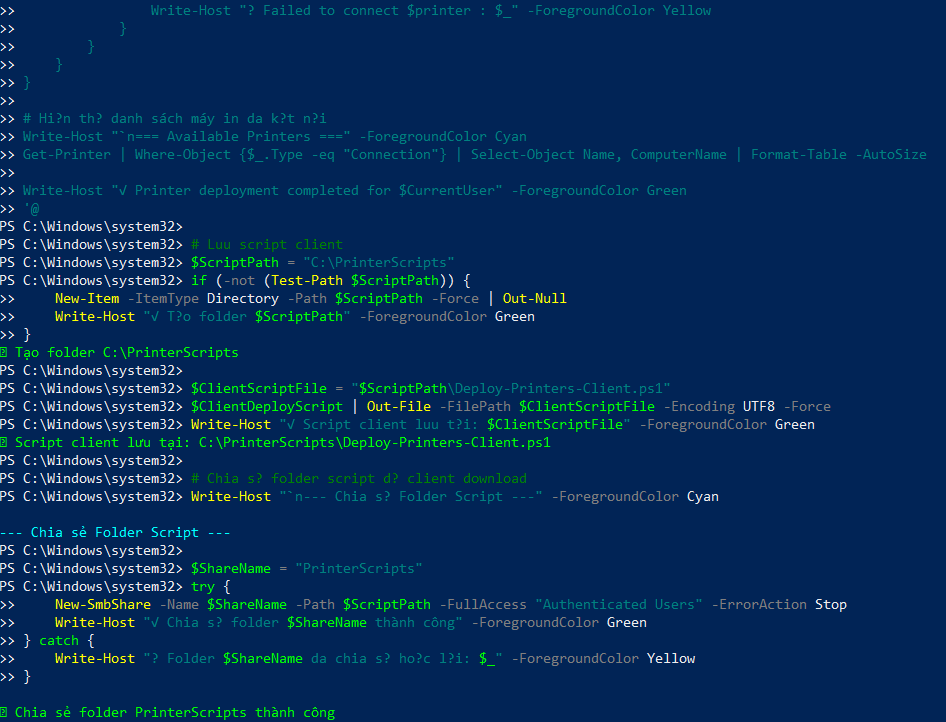
\includegraphics[width=0.7\textwidth]{./media/TẠO SCRIPT PHÂN PHỐI MÁY IN ĐẾN CLIENT(1).png}
    \vspace{-0.25cm}
    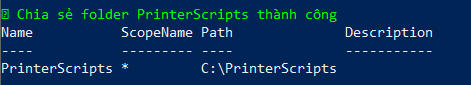
\includegraphics[width=0.7\textwidth]{./media/TẠO SCRIPT PHÂN PHỐI MÁY IN ĐẾN CLIENT(2).png}
    \caption{Tạo script phân phối máy in đến client}
    \label{fig:mirrored_vd_17}
\end{figure}

\section{Gán Script qua GPO}
\begin{lstlisting}[style=powershell]
$DomainDN = "DC=ABC,DC=local"
 
Write-Host "=== Create Department OUs ===" -ForegroundColor Cyan
 
# Create Parent OU
try {
    New-ADOrganizationalUnit -Name "PrinterGroups" -Path "OU=PrinterManagement,$DomainDN" -ProtectedFromAccidentalDeletion $false -ErrorAction SilentlyContinue
    Write-Host "[OK] OU PrinterGroups created successfully" -ForegroundColor Green
} catch {
    Write-Host "[!] OU PrinterGroups error: $_" -ForegroundColor Yellow
}
 
# Create Child OUs for each department
$DeptOUs = @(
    @{Name="Design"; Path="OU=PrinterGroups,OU=PrinterManagement,$DomainDN"},
    @{Name="Office"; Path="OU=PrinterGroups,OU=PrinterManagement,$DomainDN"},
    @{Name="Accounting"; Path="OU=PrinterGroups,OU=PrinterManagement,$DomainDN"}
)
 
foreach ($deptou in $DeptOUs) {
    try {
        New-ADOrganizationalUnit -Name $deptou.Name -Path $deptou.Path -ProtectedFromAccidentalDeletion $false -ErrorAction Stop
        Write-Host "[OK] OU '$($deptou.Name)' created successfully" -ForegroundColor Green
    } catch {
        Write-Host "[!] OU '$($deptou.Name)' error: $_" -ForegroundColor Yellow
    }
}
 
Start-Sleep -Seconds 2
 
# Link GPO to OU
Write-Host "`n=== Link GPO to OU ===" -ForegroundColor Cyan
 
$GPOConfigs = @(
    @{Name="Printers_Design"; Target="OU=Design,OU=PrinterGroups,OU=PrinterManagement,DC=ABC,DC=local"},
    @{Name="Printers_Office"; Target="OU=Office,OU=PrinterGroups,OU=PrinterManagement,DC=ABC,DC=local"},
    @{Name="Printers_Accounting"; Target="OU=Accounting,OU=PrinterGroups,OU=PrinterManagement,DC=ABC,DC=local"}
)
 
foreach ($gpo in $GPOConfigs) {
    try {
        # Note: The GPO must exist before linking
        New-GPLink -Name $gpo.Name -Target $gpo.Target -LinkEnabled Yes -ErrorAction Stop
        Write-Host "[OK] Linked GPO '$($gpo.Name)' successfully" -ForegroundColor Green
    } catch {
        Write-Host "[!] Error linking '$($gpo.Name)': $_" -ForegroundColor Yellow
    }
}
\end{lstlisting}

\begin{figure}[htbp]
    \centering
    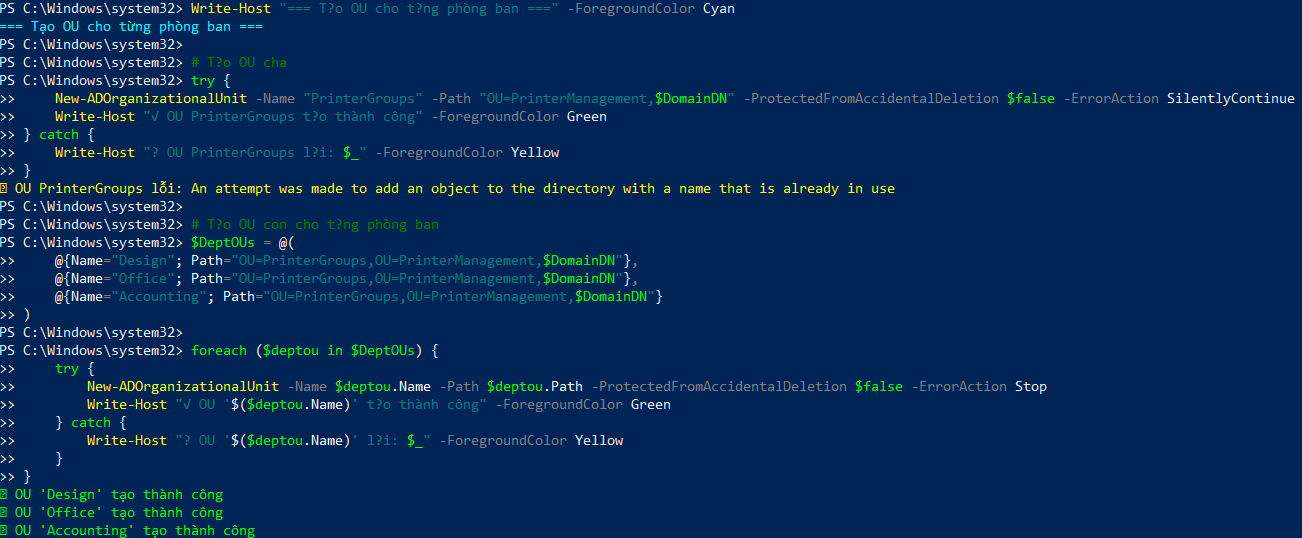
\includegraphics[width=0.68\textwidth]{./media/TẠO GROUP POLICY OBJECT (GPO) ĐỂ PHÂN PHỐI MÁY IN.png}
    \vspace{-0.2cm}
    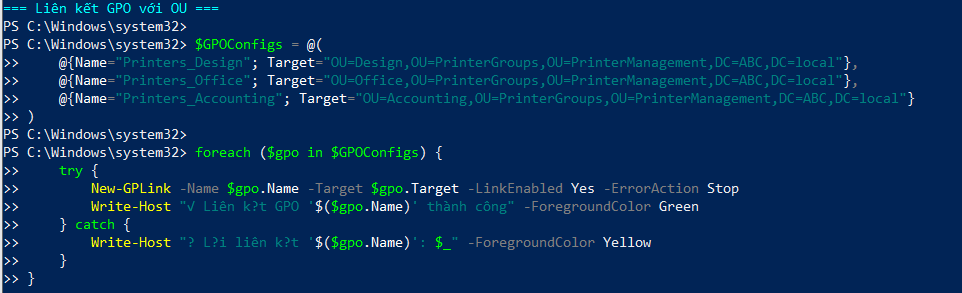
\includegraphics[width=0.68\textwidth]{./media/TẠO GROUP POLICY OBJECT (GPO) ĐỂ PHÂN PHỐI MÁY IN(1).png}
    \vspace{-0.2cm}
    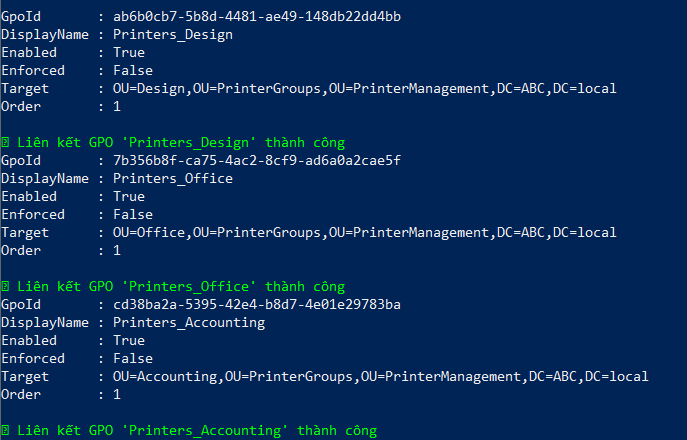
\includegraphics[width=0.68\textwidth]{./media/TẠO GROUP POLICY OBJECT (GPO) ĐỂ PHÂN PHỐI MÁY IN(2).png}
    \vspace{-0.2cm}
    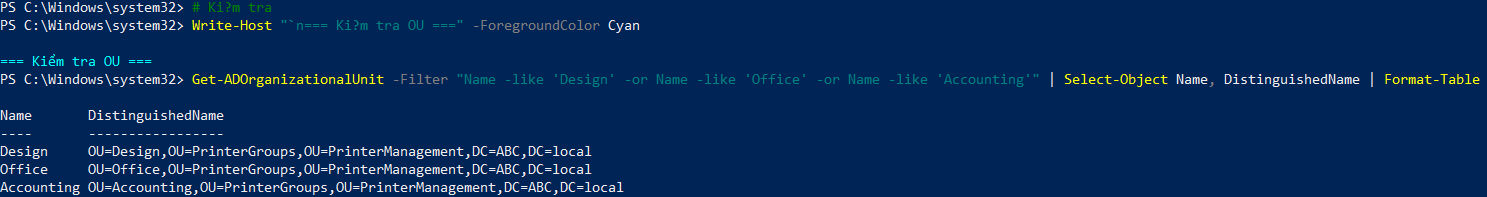
\includegraphics[width=0.68\textwidth]{./media/TẠO GROUP POLICY OBJECT (GPO) ĐỂ PHÂN PHỐI MÁY IN(3).png}
    \vspace{-0.2cm}
    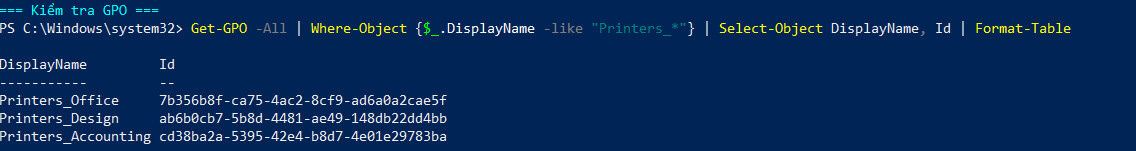
\includegraphics[width=0.68\textwidth]{./media/TẠO GROUP POLICY OBJECT (GPO) ĐỂ PHÂN PHỐI MÁY IN(4).png}
    \caption{Tạo Group Policy Object (GPO) để phân phối máy in}
    \label{fig:mirrored_vd_13}
\end{figure}

\subsection{Tạo script đọc group của user hiện tại bằng .NET}
\begin{lstlisting}[style=powershell]
$SysvolScriptPath = "C:\Windows\SYSVOL\sysvol\ABC.local\scripts\Map-DeptPrinters.ps1"
 
@'
# Map printers by department groups without AD module
 
$identity = [System.Security.Principal.WindowsIdentity]::GetCurrent()
$groups = @()
foreach ($g in $identity.Groups) {
    try {
        $name = $g.Translate([System.Security.Principal.NTAccount]).Value
        if ($name) { $groups += $name }
    } catch { }
}
 
function In-Group {
    param([string]$GroupName)
    return $groups -like "*\$GroupName"
}
 
# Debug
Write-Host "User: $($identity.Name)"
Write-Host "Groups:"; $groups | ForEach-Object { Write-Host "   $_" }
 
if (In-Group "GRP_Design") {
    Write-Host "User is in GRP_Design, mapping Design printers..."
    Add-Printer -ConnectionName "\\SRV-PRINT\PRN_Design_01" -ErrorAction SilentlyContinue
    Add-Printer -ConnectionName "\\SRV-PRINT\PRN_Design_02" -ErrorAction SilentlyContinue
}
 
if (In-Group "GRP_Office") {
    Write-Host "User is in GRP_Office, mapping Office printers..."
    Add-Printer -ConnectionName "\\SRV-PRINT\PRN_Office_01" -ErrorAction SilentlyContinue
    Add-Printer -ConnectionName "\\SRV-PRINT\PRN_Office_02" -ErrorAction SilentlyContinue
    Add-Printer -ConnectionName "\\SRV-PRINT\PRN_Office_03" -ErrorAction SilentlyContinue
    Add-Printer -ConnectionName "\\SRV-PRINT\PRN_Pool_Office" -ErrorAction SilentlyContinue
}
 
if (In-Group "GRP_Accounting") {
    Write-Host "User is in GRP_Accounting, mapping Accounting printers..."
    Add-Printer -ConnectionName "\\SRV-PRINT\PRN_Accounting_01" -ErrorAction SilentlyContinue
    Add-Printer -ConnectionName "\\SRV-PRINT\PRN_Accounting_02" -ErrorAction SilentlyContinue
}
'@ | Set-Content -Path $SysvolScriptPath -Encoding ASCII
\end{lstlisting}

\begin{figure}[htbp]
    \centering
    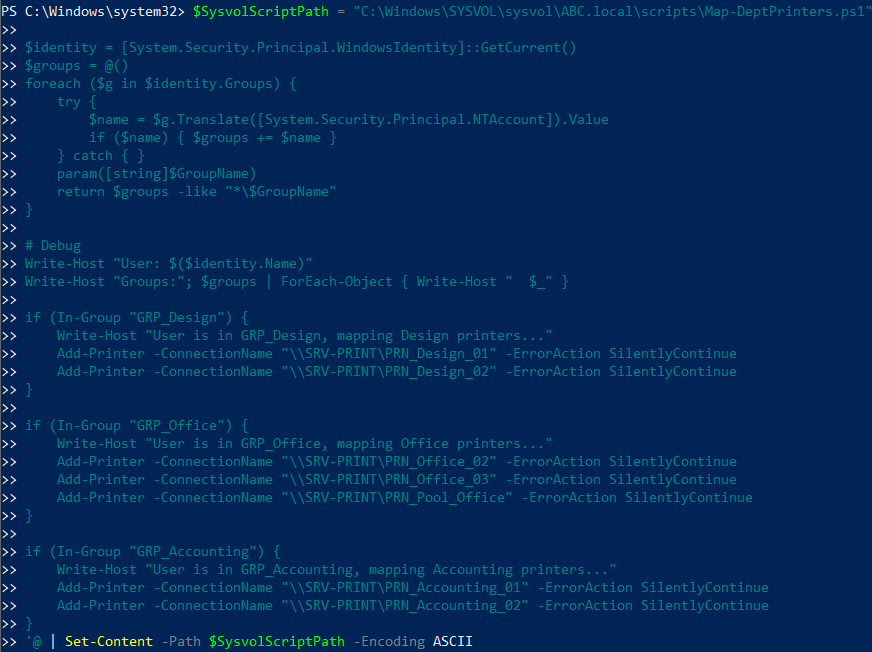
\includegraphics[width=0.75\textwidth]{./media/Tạo script đọc group của user hiện tại bằng .NET.png}
    \caption{Tạo script đọc group của user hiện tại bằng .NET}
    \label{fig:mirrored_vd_14}
\end{figure}

\subsection{Tạo GPO để chạy script khi user logon}
\begin{lstlisting}[style=powershell]
New-GPO -Name "GPO_PrinterDeploy" | Out-Null

New-GPLink -Name "GPO_PrinterDeploy" -Target "OU=Users,OU=PrinterManagement,DC=ABC,DC=local" -LinkEnabled Yes

Set-GPRegistryValue `
  -Name "GPO_PrinterDeploy" `
  -Key "HKCU\Software\Microsoft\Windows\CurrentVersion\Run" `
  -ValueName "MapPrinters" `
  -Type String `
  -Value "powershell.exe -ExecutionPolicy Bypass -File \\SRV-PRINT\sysvol\ABC.local\scripts\Map-DeptPrinters.ps1"
\end{lstlisting}

\begin{figure}[htbp]
    \centering
    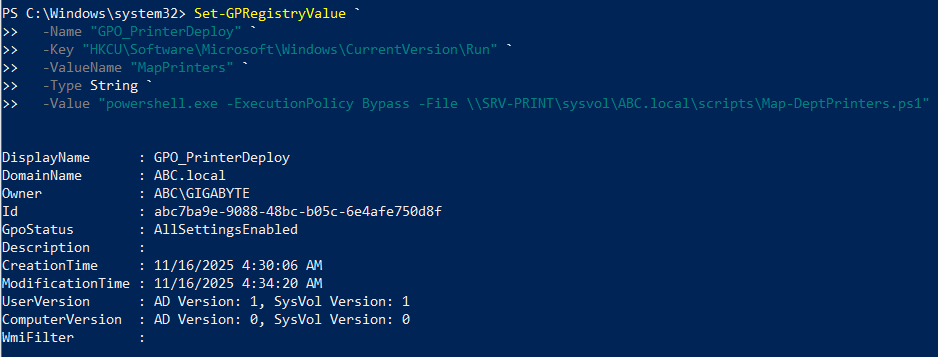
\includegraphics[width=0.75\textwidth]{./media/Tạo 1 GPO duy nhất để chạy script này khi user logon.png}
    \caption{Tạo GPO để chạy script khi user logon}
    \label{fig:mirrored_vd_115}
\end{figure}

\chapter{\textbf{Cấu hình Client tham gia Domain}}
\section{Join Domain trên Client PowerShell (As Administrator)}
Trên mỗi máy Client chạy lệnh:
\begin{lstlisting}[style=powershell]
# Dat DNS chi ve Domain Controller
$Adapter = Get-NetAdapter | Where-Object {$_.Status -eq "Up"} | Select-Object -First 1
Set-DnsClientServerAddress -InterfaceAlias $Adapter.Name -ServerAddresses "192.168.244.10"

# Join domain
$SecurePassword = ConvertTo-SecureString "ADMIN_PASSWORD" -AsPlainText -Force
$Credential = New-Object System.Management.Automation.PSCredential("abc\Administrator", $SecurePassword)
Add-Computer -DomainName "abc.local" -Credential $Credential -Force -Restart

Write-Host "Client tham gia domain thanh cong" -ForegroundColor Green
\end{lstlisting}

\subsection{Đăng nhập với Account Test}
Sau khi restart, đăng nhập với các tài khoản sau:
\begin{itemize}[topsep=2pt,itemsep=1pt,parsep=0pt]
    \item \textbf{User 1 (Phòng Thiết kế):} \texttt{ABC\textbackslash user\_design}
    \item \textbf{User 2 (Phòng Văn phòng):} \texttt{ABC\textbackslash user\_office}
    \item \textbf{User 3 (Phòng Kế toán):} \texttt{ABC\textbackslash user\_accounting}
\end{itemize}
\textbf{Password:} \texttt{Manh31102005}

\section{Kiểm tra máy in được map tự động}
Sau khi đăng nhập vào \texttt{ABC\textbackslash user\_office} với password \texttt{Manh31102005}, chạy các lệnh sau:
\begin{lstlisting}[style=powershell]
# Cho phep chay script trong phien hien tai
Set-ExecutionPolicy -Scope Process -ExecutionPolicy Bypass -Force
whoami /groups | findstr /i grp
Get-Printer | Format-Table Name,ShareName
\end{lstlisting}

\begin{figure}[htbp]
    \centering
    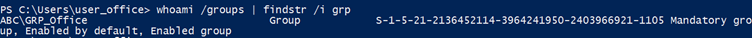
\includegraphics[width=0.75\textwidth]{./media/1.png}
    \vspace{-0.25cm}
    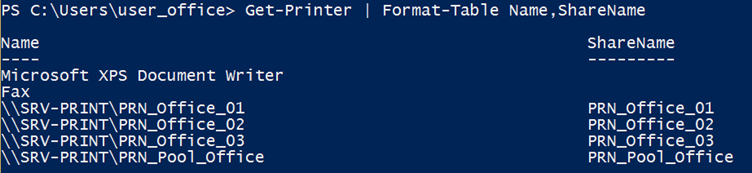
\includegraphics[width=0.75\textwidth]{./media/2.png}
    \caption{Kết quả kiểm tra sau khi đăng nhập}
    \label{fig:login_check}
\end{figure}

\subsection{Thực hiện test in}
\textbf{Bước 1:} Mở Notepad trên client

\textbf{Bước 2:} Gõ nội dung: \texttt{Test Print - user\_office}

\textbf{Bước 3:} Thực hiện in:
\begin{itemize}[topsep=2pt,itemsep=1pt,parsep=0pt]
    \item Chọn \texttt{File → Print}
    \item Chọn máy in: \texttt{\textbackslash\textbackslash SRV-PRINT\textbackslash PRN\_Office\_01}
    \item Nhấn \texttt{Print}
\end{itemize}

\textbf{Bước 4:} Kiểm tra print job:
\begin{lstlisting}[style=powershell]
Get-WmiObject -Class Win32_PrintJob |
    Select-Object Name, Document, JobId, Owner, TotalPages, Status | Format-Table -AutoSize
\end{lstlisting}

\begin{figure}[htbp]
    \centering
    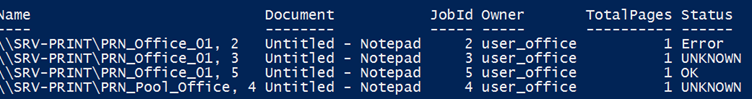
\includegraphics[width=0.8\textwidth]{./media/3.png}
    \caption{Kết quả kiểm tra print job}
    \label{fig:print_job}
\end{figure}

\subsection{Kiểm tra queue trên Server}
\begin{lstlisting}[style=powershell]
Get-PrintJob -PrinterName "PRN_Office_01" |
    Select PrinterName, JobId, JobStatus, Owner, DocumentName, SubmittedTime |
    Format-Table -AutoSize
\end{lstlisting}

\begin{figure}[htbp]
    \centering
    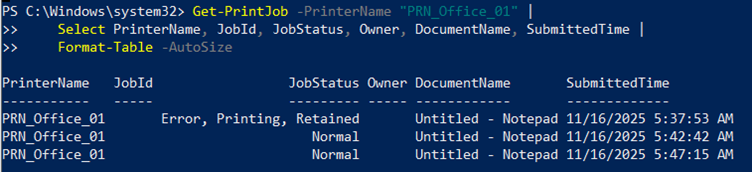
\includegraphics[width=0.8\textwidth]{./media/4.png}
    \caption{Kiểm tra queue trên server}
    \label{fig:server_queue}
\end{figure}

\subsection{Kiểm tra Event Log}
\begin{lstlisting}[style=powershell]
Get-EventLog -LogName "Print Service Log" -Newest 20
\end{lstlisting}

\begin{figure}[htbp]
    \centering
    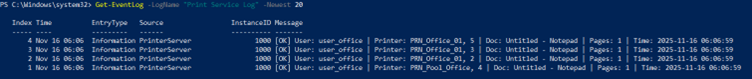
\includegraphics[width=0.8\textwidth]{./media/5.png}
    \caption{Event log của Print Service}
    \label{fig:event_log}
\end{figure}
\vspace{\baselineskip}

\chapter{\textbf{Giám sát, logging và báo cáo}}
\section{Bật Logging PrintService}
\begin{lstlisting}[style=powershell]
# Create Custom Event Log
try {
    New-EventLog -LogName "Print Service Log" -Source "PrinterServer" -ErrorAction SilentlyContinue
    Write-Host "[OK] Event Log 'Print Service Log' created successfully" -ForegroundColor Green
} catch {
    Write-Host "[!] Event Log already exists or error: $_" -ForegroundColor Yellow
}
 
# Create folder to save log files
$LogFolder = "C:\PrintLogs"
if (-not (Test-Path $LogFolder)) {
    New-Item -ItemType Directory -Path $LogFolder -Force | Out-Null
    Write-Host "[OK] Folder $LogFolder created successfully" -ForegroundColor Green
} else {
    Write-Host "[OK] Folder $LogFolder already exists" -ForegroundColor Green
}
 
# Function to log details of every print job
Function Log-PrintEvent {
    param(
        [string]$Username,
        [string]$PrinterName,
        [string]$DocumentName,
        [int]$PageCount,
        [string]$EventType = "Print Job Submitted",
        [string]$Status = "Success"
    )
    
    $Timestamp = Get-Date -Format "yyyy-MM-dd HH:mm:ss"
    
    # Write to Event Log
    try {
        Write-EventLog -LogName "Print Service Log" `
                      -Source "PrinterServer" `
                      -EventId 1000 `
                      -EntryType Information `
                      -Message "[$Status] User: $Username | Printer: $PrinterName | Doc: $DocumentName | Pages: $PageCount | Time: $Timestamp"
    } catch {
        Write-Host "[!] Error writing to Event Log: $_" -ForegroundColor Yellow
    }
    
    # Write to CSV file for long-term storage
    $CSVPath = "$LogFolder\PrintHistory.csv"
    $LogEntry = [PSCustomObject]@{
        Timestamp = $Timestamp
        Username = $Username
        PrinterName = $PrinterName
        DocumentName = $DocumentName
        PageCount = $PageCount
        EventType = $EventType
        Status = $Status
    }
    
    try {
        $LogEntry | Export-Csv -Path $CSVPath -Append -NoTypeInformation -Force -ErrorAction Stop
    } catch {
        Write-Host "[!] Error writing to CSV log: $_" -ForegroundColor Yellow
    }
}
 
Write-Host "[OK] Function Log-PrintEvent created" -ForegroundColor Green
\end{lstlisting}

\begin{figure}[htbp]
    \centering
    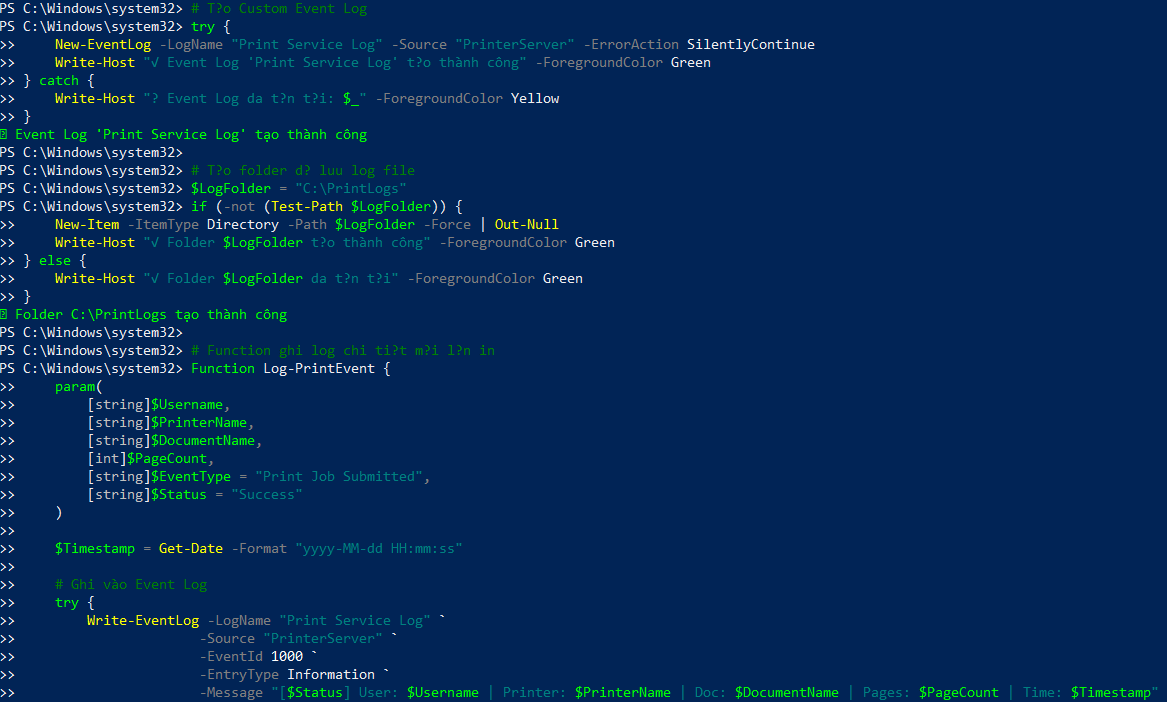
\includegraphics[width=0.72\textwidth]{./media/CẤU HÌNH LOGGING CHI TIẾT.png}
    \vspace{-0.25cm}
    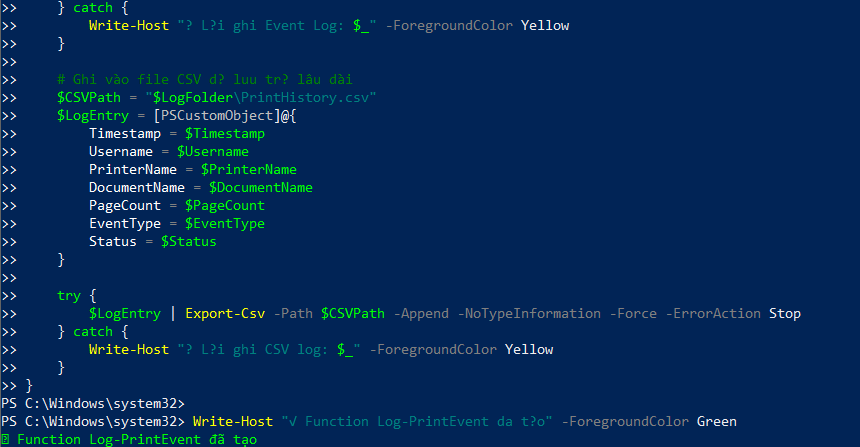
\includegraphics[width=0.72\textwidth]{./media/CẤU HÌNH LOGGING CHI TIẾT(1).png}
    \caption{Cấu hình logging chi tiết}
    \label{fig:mirrored_vd_10}
\end{figure}

\subsection{Script kiểm tra Log event}
\begin{lstlisting}[style=powershell]
# List of logged jobs (to avoid duplicates)
$global:LoggedJobs = @{}
 
# 3-second Timer
$timer = New-Object Timers.Timer
$timer.Interval = 3000
$timer.AutoReset = $true
$timer.Enabled = $true
 
Register-ObjectEvent `
    -InputObject $timer `
    -EventName Elapsed `
    -SourceIdentifier "PrintJobMonitor" `
    -Action {
 
        $jobs = Get-WmiObject -Class Win32_PrintJob -ErrorAction SilentlyContinue
 
        foreach ($job in $jobs) {
 
            # Each job has JobID + PrinterName to create a unique key
            $key = "$($job.Name)-$($job.JobId)"
 
            # If this job hasn't been logged yet -> log immediately
            if (-not $global:LoggedJobs.ContainsKey($key)) {
 
                $global:LoggedJobs[$key] = $true
 
                # Call the logging function defined previously
                Log-PrintEvent `
                    -Username $job.Owner `
                    -PrinterName $job.Name `
                    -DocumentName $job.Document `
                    -PageCount $job.TotalPages `
                    -EventType "Print Job" `
                    -Status "OK"
 
                Write-Host "Logged: $key" -ForegroundColor Green
            }
        }
    }
\end{lstlisting}

\begin{figure}[htbp]
    \centering
    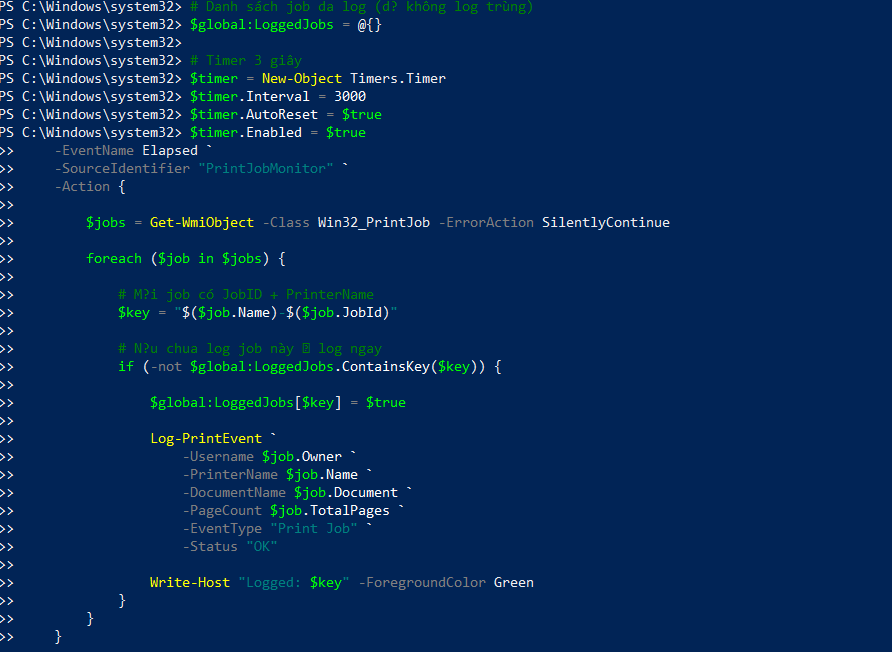
\includegraphics[width=0.99\textwidth]{./media/kiểm tra Log event.png}
    \vspace{-0.25cm}
    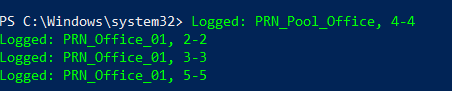
\includegraphics[width=0.99\textwidth]{./media/kiểm tra Log event(1).png}
    \caption{Kiểm tra Log event}
    \label{fig:mirrored_vd_11}
\end{figure}
\clearpage

\section{Thống kê theo người dùng và Xuất báo cáo bằng PowerShell}
\begin{lstlisting}[style=powershell]
Function Get-PrinterUsageReport {
    param(
        [string]$Username = $null,
        [DateTime]$StartDate = (Get-Date).AddDays(-30),
        [DateTime]$EndDate = (Get-Date)
    )
    
    $CSVPath = "$LogFolder\PrintHistory.csv"
    
    if (-not (Test-Path $CSVPath)) {
        Write-Host "[!] Log file not found: $CSVPath" -ForegroundColor Yellow
        return $null
    }
    
    # Read log file
    $PrintLog = Import-Csv -Path $CSVPath -ErrorAction SilentlyContinue
    if (-not $PrintLog) {
        Write-Host "[!] Log file is empty" -ForegroundColor Yellow
        return $null
    }
    
    # Filter by user and date
    $FilteredLog = $PrintLog | Where-Object {
        $LogDate = $null
        if ([DateTime]::TryParseExact($_.Timestamp, "yyyy-MM-dd HH:mm:ss", $null, [System.Globalization.DateTimeStyles]::None, [ref]$LogDate)) {
            ($null -eq $Username -or $_.Username -eq $Username) -and
            ($LogDate -ge $StartDate -and $LogDate -le $EndDate)
        }
    }
    
    if (-not $FilteredLog) {
        Write-Host "[!] No data found for the selected date range" -ForegroundColor Yellow
        return $null
    }
    
    # Calculate statistics
    $Report = $FilteredLog | Group-Object -Property Username | ForEach-Object {
        $Pages = $_.Group.PageCount | Measure-Object -Sum
        [PSCustomObject]@{
            Username = $_.Name
            TotalJobs = $_.Count
            TotalPages = $Pages.Sum
            AveragePagesPerJob = [Math]::Round($Pages.Sum / $_.Count, 2)
            MostUsedPrinter = ($_.Group | Group-Object -Property PrinterName | Sort-Object Count -Descending | Select-Object -First 1).Name
            FirstJobTime = ($_.Group | Sort-Object Timestamp | Select-Object -First 1).Timestamp
            LastJobTime = ($_.Group | Sort-Object Timestamp | Select-Object -Last 1).Timestamp
        }
    }
    
    return $Report
}
 
Function Export-PrinterReportToCSV {
    param(
        [string]$OutputPath = "$LogFolder\Report_$(Get-Date -Format 'yyyy-MM-dd_HH-mm-ss').csv",
        [int]$DaysBack = 30
    )
    
    Write-Host "Generating report for last $DaysBack days..." -ForegroundColor Cyan
    
    $StartDate = (Get-Date).AddDays(-$DaysBack)
    $Report = Get-PrinterUsageReport -StartDate $StartDate
    
    if ($Report) {
        $Report | Export-Csv -Path $OutputPath -NoTypeInformation -Force
        Write-Host "[OK] Report exported: $OutputPath" -ForegroundColor Green
        $Report | Format-Table -AutoSize
    } else {
        Write-Host "[!] No data available to export report" -ForegroundColor Yellow
    }
}
 
Function Export-UserPrinterHistory {
    param(
        [Parameter(Mandatory=$true)][string]$Username,
        [string]$OutputPath = "$LogFolder\History_$($Username)_$(Get-Date -Format 'yyyy-MM-dd_HH-mm-ss').csv"
    )
    
    Write-Host "Exporting history for user: $Username" -ForegroundColor Cyan
    
    $CSVPath = "$LogFolder\PrintHistory.csv"
    if (-not (Test-Path $CSVPath)) {
        Write-Host "[!] Log file not found" -ForegroundColor Yellow
        return
    }
    
    $PrintLog = Import-Csv -Path $CSVPath
    $UserHistory = $PrintLog | Where-Object {$_.Username -eq $Username}
    
    if ($UserHistory) {
        $UserHistory | Export-Csv -Path $OutputPath -NoTypeInformation -Force
        Write-Host "[OK] Print history for $Username exported: $OutputPath" -ForegroundColor Green
        $UserHistory | Format-Table -AutoSize
    } else {
        Write-Host "[!] No data found for user $Username" -ForegroundColor Yellow
    }
}
 
Write-Host "[OK] Report functions created" -ForegroundColor Green
\end{lstlisting}
% \begin{figure}[htbp]
%     \centering
%     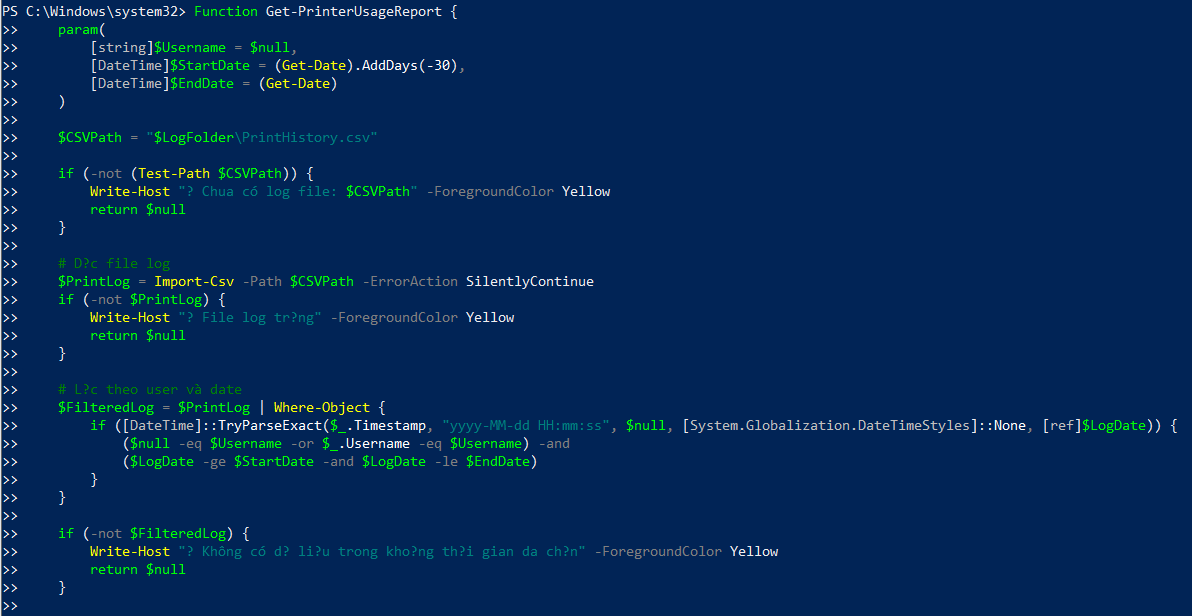
\includegraphics[width=0.68\textwidth]{./media/HÀM THỐNG KÊ VÀ XUẤT BÁO CÁO.png}
%     \vspace{-0.2cm}
%     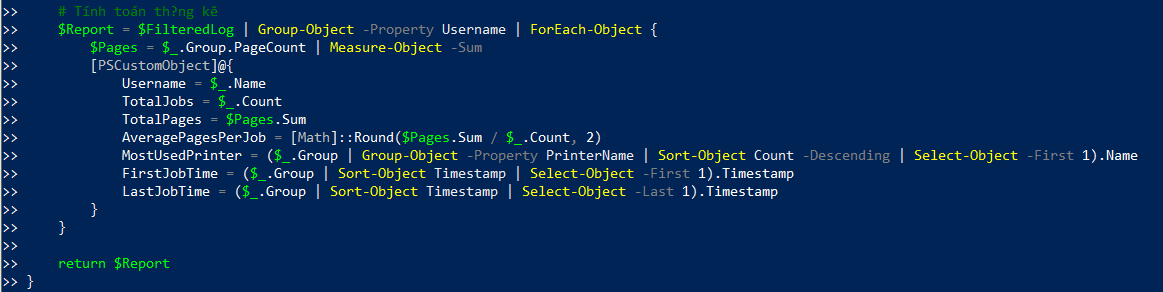
\includegraphics[width=0.68\textwidth]{./media/HÀM THỐNG KÊ VÀ XUẤT BÁO CÁO(1).png}
%     \label{fig:mirrored_vd_18}
% \end{figure}
\begin{figure}[htbp]
    \centering
    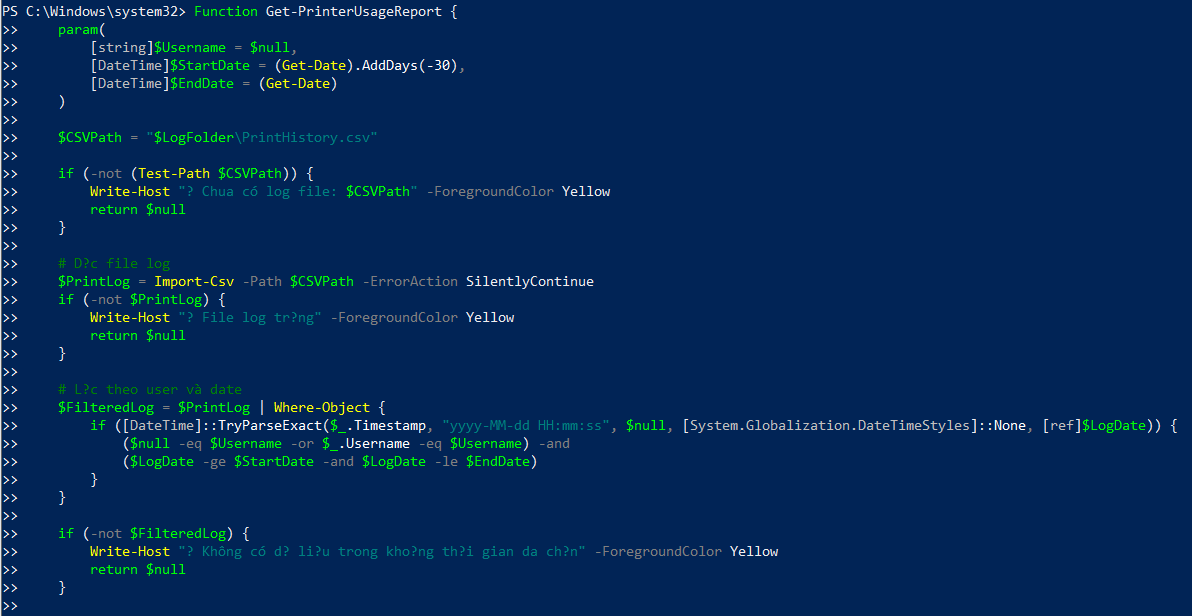
\includegraphics[width=0.68\textwidth]{./media/HÀM THỐNG KÊ VÀ XUẤT BÁO CÁO.png}
    \vspace{-0.2cm}
    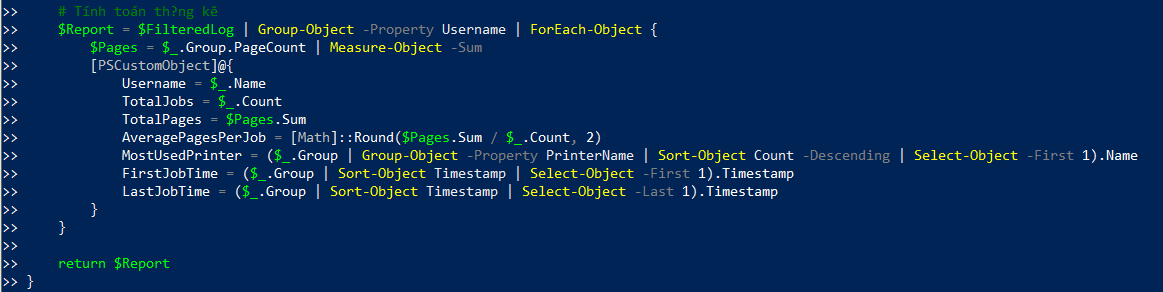
\includegraphics[width=0.68\textwidth]{./media/HÀM THỐNG KÊ VÀ XUẤT BÁO CÁO(1).png}
    \vspace{-0.2cm}
    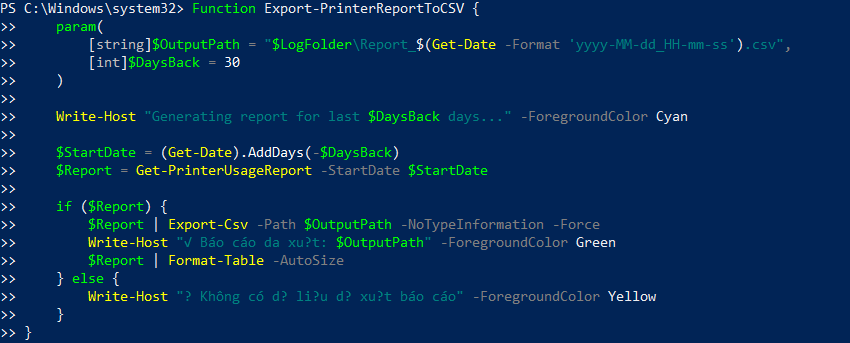
\includegraphics[width=0.68\textwidth]{./media/HÀM THỐNG KÊ VÀ XUẤT BÁO CÁO(2).png}
    \vspace{-0.2cm}
    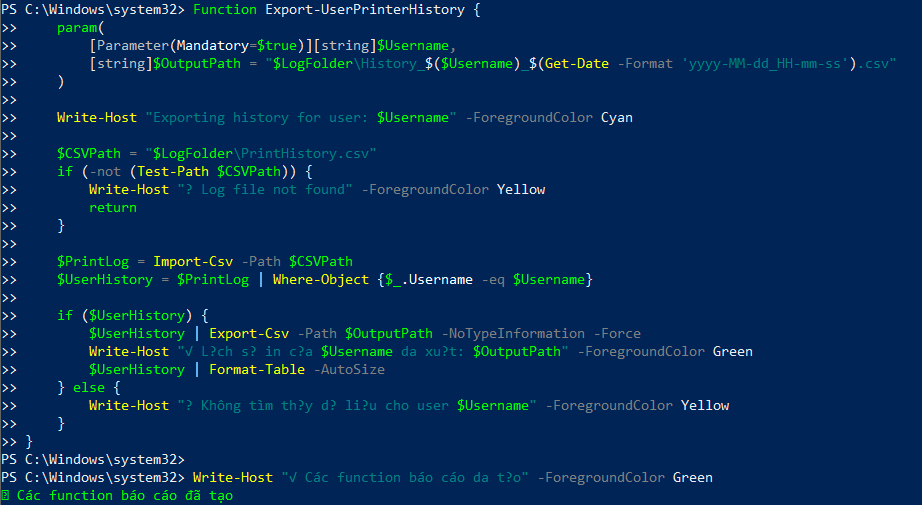
\includegraphics[width=0.68\textwidth]{./media/HÀM THỐNG KÊ VÀ XUẤT BÁO CÁO(3).png}
    \caption{Thống kê và xuất báo cáo}
    \label{fig:mirrored_vd_18}
\end{figure}
\vspace{\baselineskip}
\clearpage
\chapter{\textbf{Kiểm thử và xác thực hệ thống}}
\section{Giới thiệu}
Phần này cung cấp script tổng hợp để kiểm tra và đánh giá tình trạng hoạt động của toàn bộ hệ thống Print Server. Script thực hiện quét tuần tự qua 9 thành phần chính của hệ thống, từ cấp độ Domain Controller đến các dịch vụ và logging, giúp quản trị viên có cái nhìn toàn diện về tình trạng hệ thống trong một lần chạy.

\section{Các thành phần kiểm tra}

\subsection{Kiểm tra Domain}
Xác minh kết nối đến Active Directory Forest, hiển thị tên domain và mức độ chức năng (Forest Mode). Đây là bước đầu tiên để đảm bảo hạ tầng AD hoạt động bình thường.

\begin{lstlisting}[style=powershell]
Write-Host "`n--- 1. Kiem tra Domain ---" -ForegroundColor Cyan
try {
    $Forest = Get-ADForest -ErrorAction Stop
    Write-Host "Forest: $($Forest.Name)" -ForegroundColor Green
    Write-Host "Domain Level: $($Forest.ForestMode)" -ForegroundColor Green
} catch {
    Write-Host "Loi: $_" -ForegroundColor Red
}
\end{lstlisting}

\subsection{Kiểm tra Nhóm AD}
Liệt kê tất cả các nhóm có tiền tố "GRP\_" và đếm số lượng thành viên trong mỗi nhóm. Giúp xác nhận cấu trúc phân quyền theo phòng ban đã được triển khai đúng.

\begin{lstlisting}[style=powershell]
Write-Host "`n--- 2. Kiem tra Nhom AD ---" -ForegroundColor Cyan
$Groups = Get-ADGroup -Filter "Name -like 'GRP_*'" -ErrorAction SilentlyContinue
foreach ($group in $Groups) {
    $members = Get-ADGroupMember -Identity $group.Name -ErrorAction SilentlyContinue
    Write-Host "Nhom: $($group.Name) - Members: $($members.Count)" -ForegroundColor Green
}
\end{lstlisting}

\subsection{Kiểm tra User}
Hiển thị danh sách người dùng có tên đăng nhập bắt đầu bằng "user\_" kèm theo tên hiển thị. Xác nhận các tài khoản người dùng đã được tạo và cấu hình.

\begin{lstlisting}[style=powershell]
Write-Host "`n--- 3. Kiem tra User ---" -ForegroundColor Cyan
$Users = Get-ADUser -Filter "SamAccountName -like 'user_*'" -ErrorAction SilentlyContinue
foreach ($user in $Users) {
    Write-Host "User: $($user.SamAccountName) - $($user.DisplayName)" -ForegroundColor Green
}
\end{lstlisting}

\subsection{Kiểm tra Máy In}
Thống kê tổng số máy in trong hệ thống và số lượng máy in được chia sẻ. Đây là chỉ số quan trọng để đánh giá quy mô triển khai.

\begin{lstlisting}[style=powershell]
Write-Host "`n--- 4. Kiem tra May In ---" -ForegroundColor Cyan
$Printers = Get-Printer
Write-Host "Tong may in: $($Printers.Count)" -ForegroundColor Green
$SharedPrinters = $Printers | Where-Object {$_.Shared -eq $true}
Write-Host "May in chia se: $($SharedPrinters.Count)" -ForegroundColor Green
\end{lstlisting}

\subsection{Kiểm tra Cổng In}
Đếm số lượng cổng TCP/IP có tiền tố "IP\_", xác nhận các máy in network đã được cấu hình đúng địa chỉ.

\begin{lstlisting}[style=powershell]
Write-Host "`n--- 5. Kiem tra Cong In ---" -ForegroundColor Cyan
$Ports = Get-PrinterPort | Where-Object {$_.Name -like "IP_*"}
Write-Host "Cong in TCP/IP: $($Ports.Count)" -ForegroundColor Green
\end{lstlisting}

\subsection{Kiểm tra Printer Pool}
Xác minh máy in pool "PRN\_Pool\_Office" có tồn tại và được chia sẻ hay không. Đây là thành phần quan trọng cho việc cân bằng tải in ấn.

\begin{lstlisting}[style=powershell]
Write-Host "`n--- 6. Kiem tra Pool ---" -ForegroundColor Cyan
$PoolPrinter = Get-Printer -Name "PRN_Pool_Office" -ErrorAction SilentlyContinue
if ($PoolPrinter) {
    Write-Host "Pool: PRN_Pool_Office - Chia se: $($PoolPrinter.Shared)" -ForegroundColor Green
} else {
    Write-Host "Pool PRN_Pool_Office khong tim thay" -ForegroundColor Yellow
}
\end{lstlisting}

\subsection{Kiểm tra GPO}
Liệt kê tất cả Group Policy Objects có tên bắt đầu bằng "Printers\_" và hiển thị tên từng GPO. Xác nhận các chính sách triển khai máy in đã được tạo.

\begin{lstlisting}[style=powershell]
Write-Host "`n--- 7. Kiem tra GPO ---" -ForegroundColor Cyan
$GPOs = Get-GPO -All -ErrorAction SilentlyContinue | Where-Object {$_.DisplayName -like "Printers_*"}
Write-Host "Group Policies (Printer): $($GPOs.Count)" -ForegroundColor Green
foreach ($gpo in $GPOs) {
    Write-Host "  - $($gpo.DisplayName)" -ForegroundColor Cyan
}
\end{lstlisting}

\subsection{Kiểm tra Dịch vụ}
Kiểm tra trạng thái của 3 dịch vụ quan trọng là Print Spooler, DNS Server và Active Directory Domain Services. Hiển thị trạng thái Running hoặc Stopped với mã màu tương ứng.

\begin{lstlisting}[style=powershell]
Write-Host "`n--- 8. Kiem tra Dich vu ---" -ForegroundColor Cyan
$Services = @(
    @{Name="Spooler"; DisplayName="Print Spooler"},
    @{Name="DNS"; DisplayName="DNS Server"},
    @{Name="NTDS"; DisplayName="Active Directory Domain Services"}
)

foreach ($svc in $Services) {
    $Service = Get-Service -Name $svc.Name -ErrorAction SilentlyContinue
    if ($Service) {
        Write-Host "$($svc.DisplayName): $($Service.Status)" -ForegroundColor $(if ($Service.Status -eq "Running") {"Green"} else {"Yellow"})
    }
}
\end{lstlisting}

\subsection{Kiểm tra Logging}
Xác nhận thư mục lưu trữ log files có tồn tại và đếm số lượng file log đã được tạo. Hỗ trợ việc audit và troubleshooting sau này.

\begin{lstlisting}[style=powershell]
Write-Host "`n--- 9. Kiem tra Logging ---" -ForegroundColor Cyan
if (Test-Path $LogFolder) {
    Write-Host "Folder Logging: $LogFolder" -ForegroundColor Green
    $LogFiles = Get-ChildItem -Path $LogFolder -ErrorAction SilentlyContinue
    Write-Host "File logs: $($LogFiles.Count)" -ForegroundColor Green
} else {
    Write-Host "Folder Logging khong tim thay" -ForegroundColor Yellow
}
\end{lstlisting}

\begin{figure}[htbp]
    \centering
    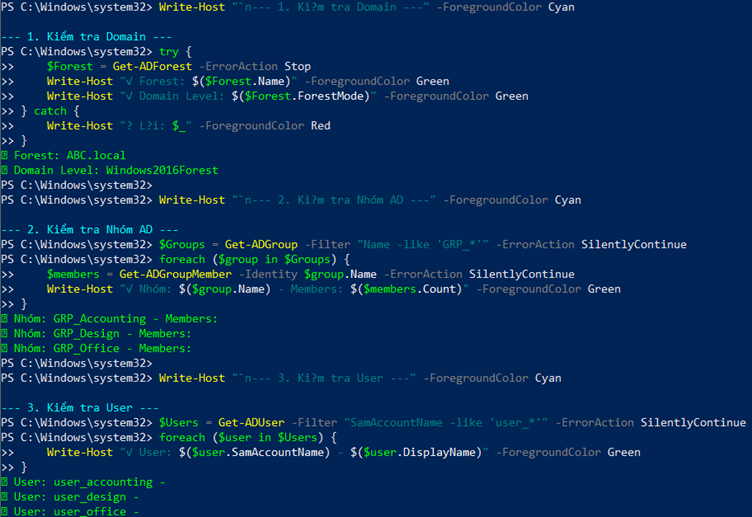
\includegraphics[width=0.65\textwidth]{./media/6.png}
    \vspace{-0.2cm}
    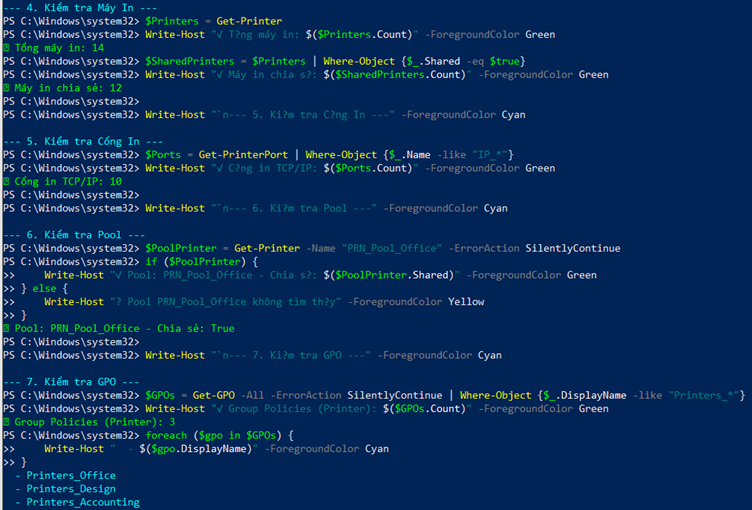
\includegraphics[width=0.65\textwidth]{./media/7.png}
    \vspace{-0.2cm}
    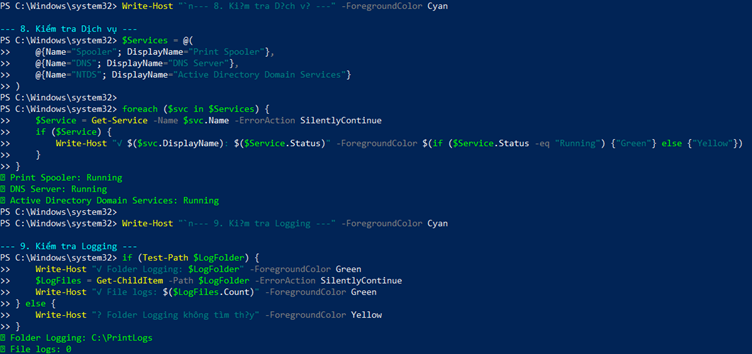
\includegraphics[width=0.65\textwidth]{./media/8.png}
    \caption{Kết quả sau khi kiểm tra}
    \label{fig:system_check}
\end{figure}

\section{Đặc điểm kỹ thuật}
Script sử dụng cơ chế xử lý lỗi (try-catch và -ErrorAction SilentlyContinue) để đảm bảo quá trình kiểm tra không bị gián đoạn khi gặp lỗi ở một thành phần. Mỗi mục kiểm tra được đánh số và có tiêu đề riêng với màu Cyan để dễ phân biệt. Kết quả hiển thị với hệ thống màu sắc: Green cho thành công, Yellow cho cảnh báo, và Red cho lỗi.

\section{Ứng dụng thực tế}
Script này được sử dụng làm công cụ kiểm tra tổng thể sau khi hoàn tất quá trình triển khai, hoặc để thực hiện health check định kỳ hàng tuần/hàng tháng. Quản trị viên có thể chạy script này để nhanh chóng đánh giá tình trạng hệ thống mà không cần kiểm tra từng thành phần riêng lẻ. Kết quả có thể được lưu lại làm báo cáo hoặc tài liệu tham khảo.

\section{Kết luận}
Phần kiểm tra toàn bộ hệ thống cung cấp một giải pháp tự động hóa cho việc đánh giá tổng thể Print Server infrastructure. Script giúp tiết kiệm thời gian, đảm bảo không bỏ sót thành phần nào và cung cấp báo cáo trực quan về tình trạng hệ thống trong thời gian thực.
\vspace{\baselineskip}

\chapter{\textbf{TROUBLESHOOTING \& GIẢI QUYẾT SỰ CỐ}}

\section{Giới thiệu}
Phần này cung cấp bộ công cụ PowerShell để kiểm tra, giám sát và xử lý sự cố cho hệ thống Print Server. Các function được thiết kế nhằm giúp quản trị viên nhanh chóng phát hiện và khắc phục các vấn đề thường gặp trong môi trường in ấn doanh nghiệp, đảm bảo hệ thống hoạt động ổn định và liên tục.

\section{Các chức năng chính}

\subsection{Get-PrinterServerStatus}
Function này kiểm tra tổng quan tình trạng Print Server bao gồm Domain Controller, các dịch vụ hệ thống (Spooler, DNS), thống kê số lượng máy in, cổng in, nhóm AD và GPO. Kết quả hiển thị dưới dạng bảng chi tiết với mã màu trực quan, giúp quản trị viên nhanh chóng nắm bắt tình trạng hoạt động của toàn bộ hệ thống và phát hiện các điểm bất thường.

\subsection{Clear-PrintQueue}
Xóa các công việc in bị treo trong hàng đợi, hỗ trợ xử lý cho một máy in cụ thể hoặc toàn bộ hệ thống. Đây là giải pháp nhanh và hiệu quả khi gặp tình trạng job in bị kẹt không thể xóa thủ công qua giao diện Windows. Function tự động đếm và báo cáo số lượng job đã được xóa thành công.

\subsection{Test-PrinterConnection}
Kiểm tra kết nối mạng đến một máy in cụ thể thông qua giao thức ICMP ping. Function này nhận vào địa chỉ IP và trả về trạng thái Online/Offline của thiết bị, giúp nhanh chóng xác định vấn đề kết nối mạng đến máy in đích.

\subsection{Test-AllPrinterConnections}
Tự động kiểm tra kết nối đến tất cả 10 máy in trong dải IP 192.168.244.201-210. Function này thực hiện ping tuần tự và hiển thị trạng thái của từng máy in, giúp quản trị viên nhanh chóng khảo sát tình trạng mạng của toàn bộ hệ thống máy in.

\subsection{Restart-PrintSpooler}
Khởi động lại dịch vụ Print Spooler với tùy chọn force để đảm bảo service được reset hoàn toàn. Đây là thao tác thường xuyên cần thiết khi máy in không nhận lệnh, hàng đợi bị treo, hoặc sau khi cài đặt driver mới. Function bao gồm xử lý lỗi để đảm bảo quá trình restart diễn ra an toàn.

\subsection{Get-PrinterDetailedInfo}
Hiển thị thông tin chi tiết về máy in (tên, máy chủ, trạng thái chia sẻ, cổng kết nối, mô tả, vị trí), cổng in (tên và địa chỉ IP), cùng với danh sách các công việc in đang chờ xử lý (người gửi, tài liệu, trạng thái, thời gian). Hỗ trợ hiệu quả cho việc troubleshooting chi tiết và audit hệ thống.

\section{Script tổng hợp}
\begin{lstlisting}[style=powershell]
Function Get-PrinterServerStatus {
    Write-Host "`n--- Trang thai Print Server ---" -ForegroundColor Cyan
    
    # Kiem tra domain controller
    try {
        $Forest = Get-ADForest -ErrorAction Stop
        Write-Host "Domain: $($Forest.Name)" -ForegroundColor Green
    } catch {
        Write-Host "Domain error: $_" -ForegroundColor Red
    }
    
    # Kiem tra dich vu Spooler
    $SpoolerStatus = Get-Service -Name Spooler -ErrorAction SilentlyContinue
    if ($SpoolerStatus.Status -eq "Running") {
        Write-Host "Print Spooler: Running" -ForegroundColor Green
    } else {
        Write-Host "Print Spooler: $($SpoolerStatus.Status)" -ForegroundColor Red
    }
    
    # Kiem tra DNS
    $DNSService = Get-Service -Name DNS -ErrorAction SilentlyContinue
    if ($DNSService.Status -eq "Running") {
        Write-Host "DNS Server: Running" -ForegroundColor Green
    } else {
        Write-Host "DNS Server: $($DNSService.Status)" -ForegroundColor Red
    }
    
    # Dem may in
    $SharedPrinters = @(Get-Printer | Where-Object {$_.Shared -eq $true})
    Write-Host "May in chia se: $($SharedPrinters.Count)" -ForegroundColor Green
    
    # Dem cong in
    $Ports = @(Get-PrinterPort | Where-Object {$_.Name -like "IP_*"})
    Write-Host "Cong in TCP/IP: $($Ports.Count)" -ForegroundColor Green
    
    # Kiem tra nhom AD
    $ADGroups = @(Get-ADGroup -Filter "Name -like 'GRP_*'" -ErrorAction SilentlyContinue)
    Write-Host "Nhom AD: $($ADGroups.Count)" -ForegroundColor Green
    
    # Kiem tra GPO
    $GPOs = @(Get-GPO -All -ErrorAction SilentlyContinue | Where-Object {$_.DisplayName -like "Printers_*"})
    Write-Host "Group Policies: $($GPOs.Count)" -ForegroundColor Green
    
    Write-Host "`n--- Chi tiet May In ---" -ForegroundColor Cyan
    Get-Printer | Select-Object Name, ComputerName, Shared, PortName | Format-Table -AutoSize
}

Function Clear-PrintQueue {
    param(
        [string]$PrinterName = $null
    )
    
    if ($PrinterName) {
        try {
            $Jobs = Get-PrintJob -PrinterName $PrinterName -ErrorAction Stop
            $Jobs | Remove-PrintJob -ErrorAction Stop
            Write-Host "Xoa $($Jobs.Count) cong viec khoi queue $PrinterName" -ForegroundColor Green
        } catch {
            Write-Host "Loi xoa queue: $_" -ForegroundColor Yellow
        }
    } else {
        try {
            $AllJobs = Get-PrintJob -ErrorAction Stop
            $AllJobs | Remove-PrintJob -ErrorAction Stop
            Write-Host "Xoa $($AllJobs.Count) cong viec tu tat ca may in" -ForegroundColor Green
        } catch {
            Write-Host "Loi xoa queue: $_" -ForegroundColor Yellow
        }
    }
}

Function Test-PrinterConnection {
    param(
        [string]$PrinterIP
    )
    
    $PingResult = Test-Connection -ComputerName $PrinterIP -Count 1 -Quiet -ErrorAction SilentlyContinue
    if ($PingResult) {
        Write-Host "May in ${PrinterIP}: Online" -ForegroundColor Green
    } else {
        Write-Host "May in ${PrinterIP}: Offline" -ForegroundColor Red
    }
}

Function Test-AllPrinterConnections {
    Write-Host "`n=== Testing All Printer Connections ===" -ForegroundColor Cyan
    $IPs = 201..210 | ForEach-Object {"192.168.244.$_"}
    foreach ($IP in $IPs) {
        Test-PrinterConnection -PrinterIP $IP
    }
}

Function Restart-PrintSpooler {
    Write-Host "Restarting Print Spooler..." -ForegroundColor Cyan
    try {
        Restart-Service -Name Spooler -Force -ErrorAction Stop
        Write-Host "Print Spooler restarted" -ForegroundColor Green
    } catch {
        Write-Host "Error restarting Print Spooler: $_" -ForegroundColor Red
    }
}

Function Get-PrinterDetailedInfo {
    Write-Host "`n--- Thong tin Chi tiet May In ---" -ForegroundColor Cyan
    Get-Printer | Select-Object Name, ComputerName, Shared, PortName, Description, Location | Format-Table -AutoSize
    
    Write-Host "`n--- Thong tin Chi tiet Cong In ---" -ForegroundColor Cyan
    Get-PrinterPort | Where-Object {$_.Name -like "IP_*"} | Select-Object Name, PrinterHostAddress | Format-Table -AutoSize
    
    Write-Host "`n--- Cong viec In Hien tai ---" -ForegroundColor Cyan
    $Jobs = Get-PrintJob -ErrorAction SilentlyContinue
    if ($Jobs) {
        $Jobs | Select-Object PrinterName, JobId, JobStatus, Owner, DocumentName, SubmittedTime | Format-Table -AutoSize
    } else {
        Write-Host "Khong co cong viec in" -ForegroundColor Yellow
    }
}

Write-Host "Cac function quan ly da tao" -ForegroundColor Green
\end{lstlisting}

\section{Ứng dụng thực tế}
Các function trong phần này được sử dụng để thực hiện kiểm tra định kỳ hàng ngày, phát hiện sớm các vấn đề tiềm ẩn về dịch vụ, kết nối mạng và hàng đợi in. Khi có sự cố xảy ra, quản trị viên có thể nhanh chóng xác định nguyên nhân gốc rễ thông qua các function kiểm tra, sau đó áp dụng giải pháp khắc phục phù hợp như restart service hoặc xóa queue.

Tất cả thao tác đều có thông báo màu sắc trực quan theo quy ước: màu xanh (Green) cho thành công, màu đỏ (Red) cho lỗi nghiêm trọng, và màu vàng (Yellow) cho cảnh báo. Điều này giúp quản trị viên dễ dàng theo dõi kết quả thực thi và đưa ra quyết định xử lý kịp thời.

\section{Kết luận}
Bộ công cụ troubleshooting này cung cấp giải pháp toàn diện cho việc quản lý và xử lý sự cố Print Server, giảm thiểu thời gian downtime và nâng cao chất lượng dịch vụ in ấn trong tổ chức. Các function có thể được tích hợp vào quy trình vận hành hàng ngày hoặc sử dụng độc lập khi cần thiết.